\documentclass[10pt,a4paper]{amsart}
\usepackage[margin=19mm]{geometry}
\usepackage{amsmath,amssymb,mathtools}
\usepackage[scr=rsfs,cal=euler]{mathalfa}
\usepackage{xfrac}
\usepackage[unicode,hidelinks,bookmarks=false]{hyperref}
\newcommand{\ie}{i.e.\ }
\newcommand{\cf}{cf.\ }
\newcommand{\resp}{respectively\ }
\newcommand{\Subsection}{\subsection}
\providecommand{\nobreakdash}{\nobreak\hbox{-}}
\setlength{\emergencystretch}{2em}
\multlinegap0pt
\usepackage{siunitx}
\usepackage{siunitx}
\usepackage{siunitx}
\usepackage{siunitx}
\usepackage{tikz}
\usepackage{float}
\usepackage{amssymb}
\usepackage{mathtools}
\usepackage{enumerate}
\usepackage{cancel}
\usepackage{siunitx}
\newtheorem{theorem}{Theorem}
\renewcommand{\le}{\leqslant}
\renewcommand{\phi}{\varphi}
\DeclareMathOperator{\xind}{x-ind}
\title{The mapping index through the lens of the cross-index}
\author{Vuong Bui, Hamid Reza Daneshpajouh, Roman Karasev}
\date{Source: arXiv:2605.12909v1 (CC BY 4.0)}
\begin{document}
\maketitle

\noindent\emph{Source and licence.} The mapping index through the lens of the cross-index. Version arXiv:2605.12909v1 (CC BY 4.0), distributed by arXiv under the Creative Commons Attribution 4.0 International licence, http://creativecommons.org/licenses/by/4.0/, as recorded in the arXiv licence metadata for this exact version and shown on the abstract page https://arxiv.org/abs/2605.12909v1. Full licence notice: \texttt{licenses/arxiv-2605.12909-CC-BY-4.0.txt}.\par\smallskip

\noindent\textit{Editorial scope.} Counted unit: the article's theorem mu(Z\_2)=1 (source0.tex lines 855--858). The article's complete original proof of it is delivered with it (source0.tex lines 860--976, one \texttt{proof} environment of 117 lines). No mathematics is written, repaired or re-derived: the statement and the proof are the article's own lines, in the article's own notation, and no retained line is substituted or re-flowed.  No further source-local context is needed: every cross-reference of every retained line resolves inside the two delivered spans.  Nothing was omitted from any retained span, so the package carries no omission record.  No retained line contains a citation, so the wrapper carries no bibliography and no bibliography entry.  The retained lines contain the article's own diagram code, which the wrapper typesets with the standard tikz packages; no image file is delivered and the package declares no asset dependency.  Editorial formatting only, in addition: an AMS \texttt{amsart} preamble that restates the article's own declarations and macros used by the retained lines, namely the environments \texttt{theorem} on separate counters, together with the standard packages those lines need.  The retained environments print in this document as Theorem 1 in order of appearance, whereas the article prints the same items with the numbering of its own full document.  The complete native source of the article as distributed in the arXiv e-print for this exact version is bundled unchanged as \texttt{sources/200461/source0.tex}.
\begin{theorem}
\label{thm: mu(Z_2)=1}
    $\mu(\mathbb{Z}_2)=1$.
\end{theorem}

\begin{proof}
We continue the previous proof with $G=\mathbb Z_2$. Denote $D(B)$ and $U(B)$ by $D$ and $U$, since we are going to use subscripts with them. Denote the elements of $G$ by $\{+1, -1\}$. The $G$-map $D\sqcup U\to G$ means a splitting $D=D_+\sqcup D_-$ and $U=U_+\sqcup U_-$ so that $D_+$ is not connected to either $D_-$ or $U_-$ in the graph of $P$, and $D_-$ is not connected to either $D_+$ or $U_+$ in the graph of $P$, and
    \[
    -1\cdot D_+=D_-, \quad -1\cdot D_-=D_+, \quad -1\cdot U_+=U_-, \quad -1\cdot U_-=U_+.
    \]
    
    Let us first split $A=A_\emptyset\sqcup A_+\sqcup A_-\sqcup A_\pm$, where $A_\emptyset$ consists of elements not above any element of $D$, $A_+$ consists of elements above some element of $D_+$ and not above any element of $D_-$, $A_-$ consists of elements above some element of $D_-$ and not above any element of $D_+$, $A_\pm$ consists of elements that are above some element of $D_+$ and above some element of $D_-$. 
    
    From transitivity it follows that the elements of $A_\emptyset$ cannot be above any element of $A_+\sqcup A_-\sqcup A_\pm$, $A_+$ cannot be above any element of $A_-\sqcup A_\pm$, $A_-$ cannot be above any element of $A_+\sqcup A_\pm$. Moreover, from transitivity no element of $A_\pm$ is below any element of $U$.   
    
    For the group action,
    \[
    -1\cdot A_\emptyset= A_\emptyset, \quad -1\cdot A_\pm= A_\pm, \quad -1\cdot A_+=A_-,\quad -1\cdot A_-=A_+.
    \]
    
    Now we invoke the $G$-equivariant map $A\to G$ that splits $A=A^+\sqcup A^-$ so that $-1\cdot A^+=A^-$ and $-1\cdot A^+=A^-$ and also splits
    \[
    A_\emptyset = A_\emptyset^+\sqcup A_\emptyset^-,\quad 
    A_+ = A_+^+\sqcup A_+^-,\quad A_- = A_-^+\sqcup A_-^-,\quad A_\pm = A_\pm^+\sqcup A_\pm^-.
    \]
    All these sets are send to each other by the action of $G$.
    
    Now set
    \[
    X_+ = D_+\sqcup A_+^+\sqcup A_\emptyset^+,\quad X_-=D_-\sqcup A_-^-\sqcup A_\emptyset^-
    \]
    and
    \[
    Y_+ = U_+\sqcup A_+^-\sqcup A_\pm^-,\quad Y_-=U_-\sqcup A_-^+\sqcup A_\pm^+.
    \]
    For the group action,
    \[
    -1\cdot X_-=X_+, \quad -1\cdot X_+=X_-,\quad -1\cdot Y_- = Y_+, \quad -1\cdot Y_+ = Y_-.
    \]

To elucidate the relations among these 12 sets defined in the proof, the Hasse diagram in Figure~\ref{fig:mu(Z_2)=1} provides a compact visual representation.

\begin{figure}[h!]
    \centering
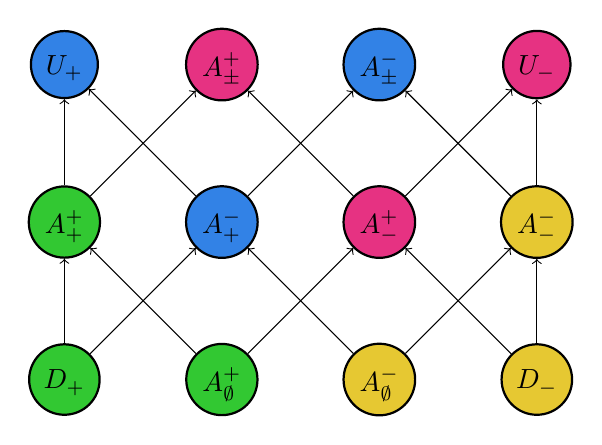
\begin{tikzpicture}[
    node style/.style={circle, draw=black, thick, font=\sffamily\bfseries, minimum size=0.8cm, text depth=0pt, align=center}
]

 
    \definecolor{myblue}{RGB}{50, 130, 230}
    \definecolor{mypink}{RGB}{230, 50, 130}
    \definecolor{mygreen}{RGB}{50, 200, 50}
    \definecolor{myyellow}{RGB}{230, 200, 50}

    % --- LAYER 1 (Top, y=6) ---
    \node[node style, fill=myblue] (U_plus) at (0, 6) {\(U_+\)};
    \node[node style, fill=mypink] (A_bar_plus) at (2, 6) {\(A_{\pm}^{+}\)};
    \node[node style, fill=myblue] (A_bar_minus) at (4, 6) {\(A_{\pm}^{-}\)};
    \node[node style, fill=mypink] (U_minus) at (6, 6) {\(U_{-}\)};

    % --- LAYER 2 (Middle, y=4) ---
    \node[node style, fill=mygreen] (A_plus_green) at (0, 4) {\(A_+^+\)};
    \node[node style, fill=myblue] (A_plus_blue) at (2, 4) {\(A_+^{-}\)};
    \node[node style, fill=mypink] (A_bar_plus_mid) at (4, 4) {\(A_{-}^{+}\)};
    \node[node style, fill=myyellow] (A_minus_yellow) at (6, 4) {\(A_{-}^-\)};

    % --- LAYER 3 (Bottom, y=2) ---
    \node[node style, fill=mygreen] (D_plus) at (0, 2) {\(D_+\)};
    \node[node style, fill=mygreen] (A_empty_green) at (2, 2) {\(A_{\emptyset}^{+}\)};
    \node[node style, fill=myyellow] (A_empty_yellow) at (4, 2) {\(A_{\emptyset}^{-}\)};
    \node[node style, fill=myyellow] (D_minus) at (6, 2) {\(D_-\)};


\draw[->] (A_plus_green) -- (U_plus);
\draw[->] (A_plus_blue) -- (U_plus);

\draw[->] (A_plus_green) -- (A_bar_plus);
\draw[->] (A_bar_plus_mid) -- (A_bar_plus);

\draw[->] (A_plus_blue) -- (A_bar_minus);
\draw[->] (A_minus_yellow) -- (A_bar_minus);

\draw[->] (A_bar_plus_mid) -- (U_minus);
\draw[->] (A_minus_yellow) -- (U_minus);

% Layer 2 to Layer 3
\draw[->] (D_plus) -- (A_plus_green);
\draw[->] (A_empty_green) -- (A_plus_green);

\draw[->] (D_plus) -- (A_plus_blue);
\draw[->] (A_empty_yellow) -- (A_plus_blue);

\draw[->] (A_empty_green) -- (A_bar_plus_mid);
\draw[->] (D_minus) -- (A_bar_plus_mid);

\draw[->] (A_empty_yellow) -- (A_minus_yellow);
\draw[->] (D_minus) -- (A_minus_yellow);

\end{tikzpicture}
    \caption{A Hasse diagram showing the 12 subsets $A_*^*$, $D_*$, $U_*$ and possible arrows between them}
    \label{fig:mu(Z_2)=1}
\end{figure}
    
    Observe that $X_+$ is not connected to $X_-$, because $D_+$ is not connected to $D_-$, $D_+$ is not connected to $A_\emptyset$ or $A_-$, $D_-$ is not connected to $A_\emptyset$ or $A_+$, $A^+$ is not connected to $A^-$.
    
    $Y_+$ is not connected to $Y_-$, because $U_+$ is not connected to $U_-$, $U_+$ is not connected to $A_\pm$ or $A_-$, $U_-$ is not connected to $A_\pm$ or $A_+$, $A^+$ is not connected to $A^-$.
    
    No element of $X_+\sqcup X_-$ is above an element of $Y_-\sqcup Y_+$. Let us show this assuming without loss of generality that $x\in X_+$:
    \begin{itemize}
    \item
    $x\in D_+$ cannot be above any element of $A$ and above any element of $U$;
    \item
    $x\in A_+^+$ cannot be above any element of $U$ or above any element of $A^-\cup A_\pm\cup A_-$;
    \item
    $x\in A_\emptyset^+$ cannot be above any element of $U$ or above any element of $A_+\sqcup A_-\sqcup A_\pm$ or above any element of $A_\emptyset^-$.
    \end{itemize}
    So we construct a $G$-equivariant monotone map
    \[
    \phi(X_+) = (+,0),\quad \phi(X_-) = (-,0),\quad \phi(Y_+) = (+,1),\quad \phi(Y_-) = (-,1)
    \]
    that certifies $\xind P\le 1$.
\end{proof}

\end{document}
